% This file is iccc.tex.  It contains the formatting instructions for and acts as a template for submissions to ICCC.  It borrows liberally from the AAAI and IJCAI formats and instructions.  It uses the files iccc.sty, iccc.bst and iccc.bib, the first two of which also borrow liberally from the same sources.

\documentclass[letterpaper]{article}
\usepackage{iccc}
\usepackage{times}
\usepackage{helvet}
\usepackage{courier}
\usepackage{graphicx}
\usepackage{amsmath}
\usepackage{amssymb}
\usepackage{booktabs}
\usepackage{algorithmic}
\usepackage{algorithm}

\graphicspath{ {images/} }

\newcommand\mydots{\hbox to .75em{.\hss.\hss.}}

\pdfinfo{
/Title (Three Artificial Intelligence Tasks for Data-Driven Musical Metacreativity in Pop Music)
/Subject (Proceedings of ICCC)
/Author (Anonymized)}
%/Author (Paul Bodily)}
% The file iccc.sty is the style file for ICCC proceedings.
%
\title{Three Artificial Intelligence Tasks for Data-Driven Musical Metacreativity in Pop Music}
%\author{Paul Bodily, Benjamin Bay, and Dan Ventura\\
%Computer Science Department\\
%Brigham Young University\\
%Provo, UT 84602  USA\\
%paulmbodily@gmail.com, benjamin.bay@gmail.com, ventura@cs.byu.edu\\
%}
\author{\emph{Anonymized}\\
\\
\\
\\
\\}
\setcounter{secnumdepth}{0}

\begin{document} 
\maketitle
\begin{abstract}
\begin{quote}
People and computers alike draw on artificial intelligence capabilities in order to learn models of styles, patterns, and structures that are present in lyrical pop music. Though many systems exist for analyzing this metadata in related domains, we examine three problems that are particular to comprehending lyrical pop music that have not received attention: automated key inference from melody; inference of verse-chorus segmentation; and rhyme scheme inference. For each of the three problems we A) define the problem and discuss its significance, B) describe methods for solving the problem, and C) report results for the methods described. We discuss how these and other AI hurdles in pop music analysis represent fundamental challenges to being able to effectively develop data-driven solutions for musical metacreativity. 
\end{quote}
\end{abstract}

\section{Introduction}
Aspiring composers and musicians rely on a host of intelligent capabilities in order to improve their art. They listen to thousands of hours of music, analyzing styles, patterns, and structures in order to more intelligently construct their own music.

Likewise systems devoted to musical metacreativity (MUME) require a host of artificial intelligence capabilities to analyze training examples, developing models that similarly capture styles, patterns, and structures. Several such systems have been developed. For example, Pachet's use of Markov models to generate novel jazz leadsheets. And so on.

As a counterpart to these systems, there are several computational creative systems that use artificial intelligence to analyze metafeatures in poetry. For example, Hirjee's system that analyzes rhyme schemes to generate rap. 

However, the realm of lyrical music that lies at the intersection of these domains has been almost completely overlooked in the research community. This is surprising for a few reasons. First, lyrical music represents the most popular form of music in industry\footnote{see this website that says pop music is most popular}, suggesting there is a great opportunity for large impact in this field. Second, there are a number of interesting AI problems that, for various reasons, are unique to this intersection.

We propose to look at three such problems in this paper. These three tasks in AI are fundamental to the creative learning process of human composers and play similarly important roles for effective learning in musical metacreativity systems.

We first discuss each of the three problems. We then discuss the methods by which we attempt to solve each problem. Following a section reporting experimental results, we discuss how these and other AI tasks are fundamental to MUME systems.

\subsection{Problem \#1: Automated Key Inference From Melody}

Humans possess the uncanny ability to listen to a friend singing or whistling a melody without any harmony and immediately infer the key or tonality in which the melody is being articulated. This allows the listener to better understand the roles and relationships between notes in the melody in order to make infer subsequent mental models of how tonal melodies are structured.

Though several systems exist which infer key from polyphonic audio \cite{A,B,C} or from polyphonic or harmonized symbolic music \cite{D,E,F}, we are aware of no system or model that infers key from a monophonic melodic line. The need for such a system is uniquely motivated by our interest in the pop music domain. Although a music system can't (yet) listen to a person humming or whistling a tune, much of what data is available online for lyrical pop music is in the form of monophonic unharmonized melodies (e.g., Karoake MIDI), and much of the data contains either missing or erroneous key signature metadata. Besides the data-driven need for a system that infers key signature from melody, there remains the broader philosophical interest: if humans can infer key from melody, how well can we teach a computer to do it?

%%%% COPIED %%%%%%
\noindent The key or tonic is a root pitch and modality (major or minor) which forms the structural basis for tonal music. This tonality provides a context within which ``the melodic and harmonic unfolding of a composition takes place'' \cite{vos1996parallel}. Even the untrained ear appreciates the structure, dissonance, and resolution that tonality provides.

Western pop music in particular presents an interesting case study because unlike much of its classical counterpart, pop songs regularly and deliberately break rules of traditional modulation and are often found to end on chords that are either unresolved or are entirely unrelated to the key in which the rest of the song is written.

There is a profound irony in the contrast between knowing how and being able to explain how to infer a song's key. Expert musicians routinely and accurately infer a song's key. However the best description for their methodology often goes no further than to find the key that ``feels'' right, provides a sense of ``finish'', or the key where the song ``lands''.

In this context it has commonly been supposed that one need simply find the key which minimizes the total number of accidentals in a song. Part of our purpose is to test this hypothesis by comparing this approach with several machine learning algorithms.

Harmony plays an integral role in determining a song's key. However, we hypothesize that the melody alone is sufficient in most cases to determine a song's key. We test this hypothesis on a dataset of 480 pop melodies in MIDI format.

\section{Related Work}

Several previous studies have examined key inference in various contexts, though to our knowledge our is the first attempt to do so using solely melodies and in the pop music domain.

Krumhansl matches the relative frequencies and durations with which tones are sounded (which she terms a \emph{tonal hierarchy}) of a song against the known tonal hierarchies of each key \cite{krumhansl2001cognitive}. This algorithm was applied to infer keys for compositions from three classical composers, Bach, Chopin, and Shostakovich. 

The key-finding algorithm of Longuet-Higgins and Steedman successively eliminates keys based on the presence or absence of the song's notes in each of the major and minor scales \cite{longuet1971interpreting}. Holtzman (1977) infers key from the prevalence of common key-defining intervals (e.g., triads, tonic-fifths, tonic-thirds). Both algorithms applied their algorithm to Bach's \emph{Well-Tempered Clavier}.

Hu and Saul take an LDA approach to key-finding, looking for common co-occurrences of notes in songs. Their model essentially treats keys like topics. They then model songs as a random mixture of key-profiles, allowing them to track modulations \cite{hu2009probabilistic}. Temperley interprets the traditional key-profile model as a Bayesian probabilistic model and discusses the implications of the connection between these two models \cite{temperley2002bayesian}. All applications of the model are on the Kostka-Payne corpus, a collection of textbook excerpts of tonal music. Vos and Van Geenen present a parallel search key-finding algorithm for single-voiced music. A song's notes are evaluated against both the scalar and the chordal structures of each key. They demonstrate the model's effectiveness on Bach's Well-Tempered Clavier \cite{vos1996parallel}. Zhu et al. present a method for key estimation in acoustic pop and classical music \cite{zhu2005music}. Their method performs marginally higher with pop music than classical music. 

Much recent work has been devoted to inferring key from acoustic music. Shenoy et al. outline a rule-based algorithm for finding key from acoustic musical signals using chroma based frequency analysis and chord progression patterns \cite{shenoy2004key}. Mauch and Dixon infer chords and key simultaneously from audio \cite{mauch2010simultaneous}. Chafe et al. extract symbolic music from audio from which meter and key are inferred (in that order) \cite{chafe1982toward}. The key-recognizer assumes that rhythmic and melodic accent points are significant features for inferring key.

Several methods have been presented for identifying key signature. They have been used mostly in Classical music. Pop music uses different modulations and is unique in that often the song finishes on a chord other than the key the song is in. No studies were found to examine key inference in pop melodies.

%%%END COPIED%%%

\subsection{Problem \#2: Verse-Chorus Inference}

One of the most natural inferences that a human listener makes while listening to a pop song is the subconscious annotation of \emph{global structure}, meaning verse-chorus segments. More broadly these segments may include intros, verses, interludes, prechoruses, choruses, bridges, and outros. In general, the listener is keenly aware of where segment boundaries take place and which segment is currently playing. This inference is important to building expectation, creating surprise, and evoking an effective range of emotion (e.g., tension and release) that are fundamental to musical creativity.

Unfortunately what symbolic pop music data \emph{is} available does not reliably nor consistently annotate global structure, and therefore it must be somehow inferred by MUME systems, as well. There are relatively few systems that have been published which consider how to automatically infer this global structure in lyrical pop music. This challenge is unique to lyrical pop music because of how the lyrics contribute to this structure.

It should be noted that solutions to this problem serve a wider purpose: repetitions in viewpoints such as melody, harmony, and lyrics exist beyond those defined by verse-chorus segmentation. Indeed, the ability to infer global structure is really a question of how to identify musical motifs generally. Motif-finding is hardly a new endeavor and much groundwork has been done particularly in bioinformatics to develop motif-finding algorithms in sequential data \cite{NW, SW}.

\subsection{Problem \#3: Rhyme Scheme}

With few exceptions lyrical music is popular because of the creativity evoked in the rhyming patterns within the lyrics. Much about rhyming resembles a sort of simple mind game: rhymes naturally serve to build anticipation in the listener's mind about what is coming next; the listener is seemingly invited to guess what word will complete the rhyme; and simply identifying when rhyming words occur provides the listener with a sense of sharing in the deeper understanding communicated in the composition. 

How rhymes are completed is only one half of how they are used in creativity. How the rhyme scheme is structured is itself an artefact of creativity that listeners naturally infer, evaluate, and appreciate.

Though related to analyzing rhyme in other non-musical contexts (e.g., poetry), rhyming in pop music is unique because the perception of rhyme is dramatically impacted by complex interactions between the lyrics and the melody (both pitch and rhythm).

\section{Methods}
\subsection{Automated Key Inference From Melody}

%%%COPIED

We collected 480 melodies from 278 pop artists representing music spanning several decades (see Figure~\ref{tab:data_summary}). Songs were compiled from several online MIDI databases and keys were manually labeled. We were pleased to find that every key was represented by at least two songs (see Figure~\ref{fig:key_distribution}). Only songs with a single key were selected for our experiments. Melodies notes were isolated from the MIDI files. 


\begin{figure}
  \centering
 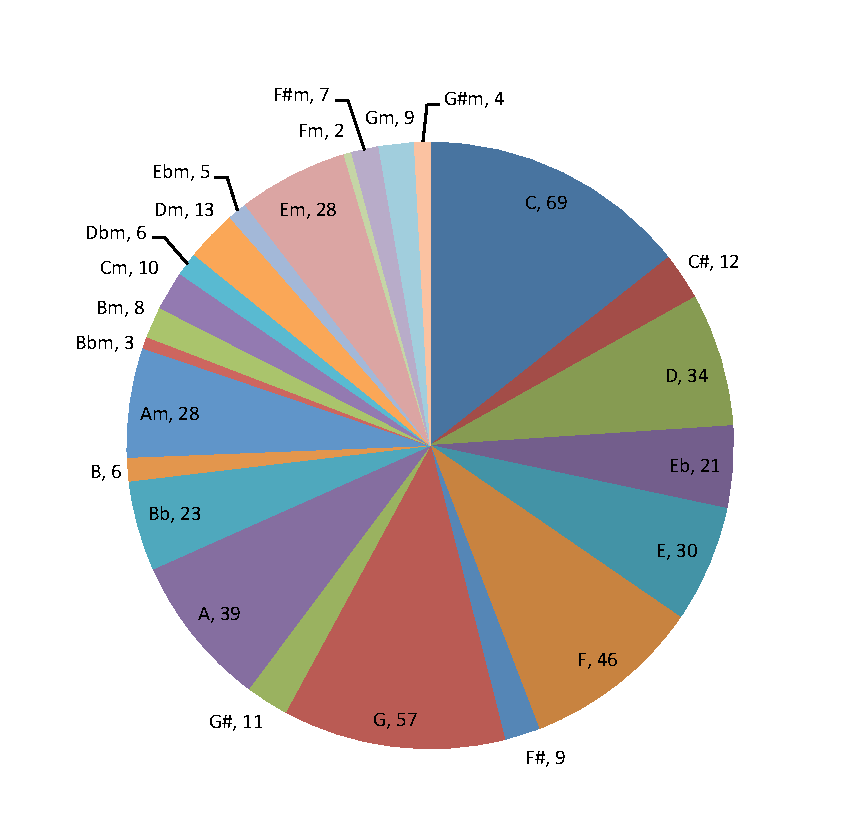
\includegraphics[width=.4\textwidth]{./key_distribution.pdf}
  \caption{\emph{Key distribution of pop melodies}. Every key is represented at least twice in the subset of melodies. In general keys with fewer sharps and flats are more highly represented.}
  \label{fig:key_distribution}
\end{figure}

\begin{table}[]
\centering
\caption{Highly Represented Pop Artists}
\label{tab:data_summary}
\begin{tabular}{@{}lc@{}}
\toprule
Artist & \# of songs\\ \midrule
beatles	& 28 \\
elvis presley	& 13 \\
kiss	&	11 \\
madonna	&	8 \\
eagles	&	6 \\
aerosmith	&	6 \\
elton john	&	6 \\
u2	&	6 \\
beach boys	&	5 \\
michael jackson	&	5 \\
pink floyd	&	5 \\
bobby vee		&	5 \\
adele	&	5 \\
queen	&	4 \\
kinks		&	4 \\
\end{tabular}
\end{table}

We compared the accuracy of 4 traditional and 5 machine learning methods on the task of inferring key signature for pop melodies. For the machine learning methods, we used 10-fold cross validation for training and testing.

\emph{Minimize Accidentals By Count}. This algorithm represents the common theory that the best key is that which minimizes the number of resulting accidentals.

\emph{Minimize Accidentals By Duration}. Similar to the previous method but finds the key which minimizes the total duration of accidentals.

\emph{RMSE of Pitch Count Profiles}. Similar to the method followed by \cite{krumhansl2001cognitive} and others, we generated pitch profiles. Rather than generate profiles for each major and minor key, we chose to generate a single profile for all major keys and a second for all minor keys. This decision is based on the assumption that the variation in pitch distribution varies very little (if at all) as compared to the distributional variation between the major and minor modes. Major and Minor mode pitch profiles were generated from the pitch counts in training instances normalized to either the C major or A minor keys depending on the whether the instance was major or minor. A pitch profile is created for each test instance, transposed into each of the 12 possible keys. Each transposed profile is compared to both the major and minor generic pitch profiles using root mean squared error (RMSE). The transposed pitch profile and the major/minor pitch profile with the minimum RMSE value are used to infer key and modality.

\emph{RMSE of Pitch Duration Profiles}. Similar to the previous method but pitch profiles are generated from pitch durations rather than mere counts (see Figure~\ref{fig:pitch_profiles}). 

n\emph{-gram Models}. An n-gram model calculates the probability of the next token given some context window of length \emph{n}. These probabilities are learned from the sequence of notes in the training instances and then used to calculate the probability of note sequences in the test instances. We trained \emph{n}-gram models for values of n from 1 to 5, using Laplace smoothing and a pseudocount alpha value of 1. For each value of \emph{n} a single \emph{n}-gram model was trained for melodies in major keys and another for melodies in minor keys. Probabilities were normalized across both models. Training instances were than transposed and scored by each trained model. The transposition and model which maximized the probability of the training instance determined the key and modality.

In addition to the methods described above, we also report accuracy from three other sources. The baseline accuracy represents the approach of always guessing the most common class. MIDI Annotations refers to the key signature that was originally given in the MIDI file (if any was provided).

Lastly we report the accuracy of a third-party MIDI-reader called MuseScore. Our interest in this problem was initially sparked by the need to normalize lyricized pop music data for compositional analysis. The most ready source for data of this type was found to be karaoke files in MIDI format (also referred to as the KAR format). Insofar as MIDI is a format concerned primarily with generating audio, many such files fail to include (accurate) information about key or time signature, thus motivating the need to infer this information from the notes themselves. This functionality is built in with varying success to many programs which render MIDI files as sheet music. MuseScore (version 2.0.3) is one such program and we include the accuracy of MuseScore's inferred key-signature in our results for comparison. 

\begin{figure}
  \centering
 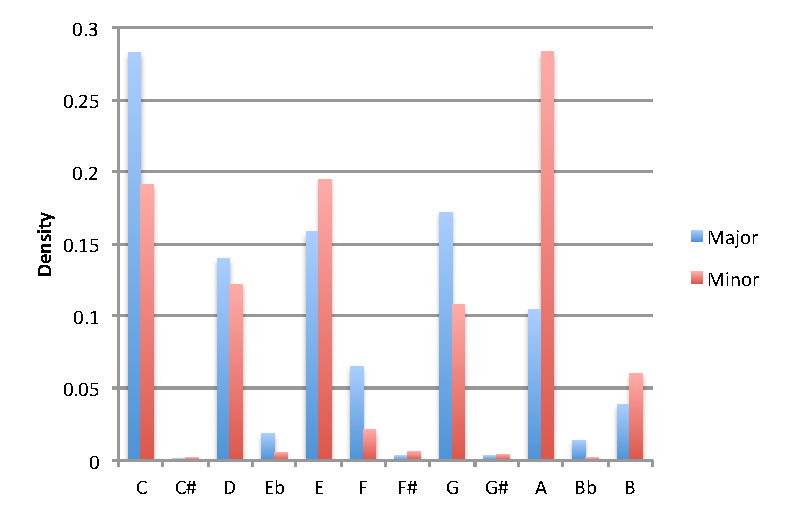
\includegraphics[width=.5\textwidth]{./PitchProfilesWeighted.pdf}
  \caption{\emph{Weighted Major/Minor Pitch Profiles}. Profiles are based on the duration of pitches in each of the major and minor modes. Profiles for major keys (blue) have been normalized to C major and those for minor keys (red) to A minor. Note that the A pitch is relatively more frequent for minor keys (where it functions as the tonic) than for major keys (where it functions as the 6th from the root). Likewise the G pitch is relatively more frequent for major keys (where it functions as the dominant) than for minor keys (where it functions as the 7th from the root).}
  \label{fig:pitch_profiles}
\end{figure}

%%%END COPIED

\section{Results}

Results are shown in Table~\ref{tab:results}. We report accuracy both for inferring the key and for inferring the key signature. Inasmuch as key signature is a more generic classification of key (e.g., C major and A minor both have a key signature with no flats or sharps), accuracy for key signature will always be better than accuracy for key.
\begin{table}[]
\centering
\caption{Key Finding Accuracy for Pop Melodies}
\label{tab:results}
\begin{tabular}{@{}lll@{}}
\toprule
Method & Key & Key Signature \\ \midrule
Baseline (C)	&	0.144 	&	0.202 \\
MIDI	Annotations		&	n/a		&	0.483 \\
MuseScore	&	n/a		&	0.746 \\ \midrule
Minimize Accidentals	 by Count	&	0.494 &		0.660 \\
Minimize Accidentals	 by Duration	&	0.490 &		0.665 \\
RMSE of Pitch Count Profiles	&	0.606	&	0.796	\\
RMSE of Pitch Duration Profiles	&	0.613	&	0.765	\\ \midrule
Unigram model    	&	0.629	& 0.815       \\
Bigram model		&	0.654	&	0.883	\\
Trigram model		&	0.679	&	0.883	\\
4-gram model		&	\emph{0.729} &	\emph{0.896}	\\
5-gram model		&	0.700 &	0.885              \\ \bottomrule
Human (``I know this song'')		&	0.846	&	0.865	\\
Human (``Sounds familiar'') 		&	0.75 &	0.786	\\
Human (``I don't know this song'')		&	0.676 &	0.815              \\ \midrule
Human Average		&	0.719 &	0.822              \\ \bottomrule
\end{tabular}
\end{table}

%people somehow use memory of a song to help them infer the key of its melody when played in isolation

\subsection{Verse-Chorus Inference}

%%%%%%%%%%%%COPIED%%%%%

We have endeavored to solve this problem using an alignment approach in order to perform unsupervised annotation of a large corpus of unlabeled chord sheets. Identifying repetitive elements or motifs in sequences has been widely-studied in the fields of bioinformatics and to a lesser extent in natural language. The Needleman-Wunsch (NW) algorithm is designed to discover optimal end-to-end alignments of sequence pairs. The Smith-Waterman (SW) algorithm varies slightly from the NW algorithm in that it is designed to find areas of high local-alignment.

We have developed a sequence alignment approach for identifying verse-chorus and rhyme-scheme structures in chord sheets. Our approach first uses pairwise Multiple Sequence Alignment (MSA) using the NW algorithm to identify and validate the actual song content in the chord sheets. Once the song content is validated, we use a novel hierarchical alignment approach loosely similar to a SW alignment of NW sub-alignments to identify choruses from repetitive subsequences of lyrics (and chords?) and verses from repetitive subsequences of chords. For this purpose we have developed a Generalized Alignment Module (GAM) which is capable of aligning sequences of any type (e.g., strings, chords, alignments, phonemes). Finally we use our GAM to align phonemes for the purpose of rhyme scheme detection. We report the results of our approach on a set of 100 chord sheets that have been manually labeled and outline our vision for how this work might be extended.

We first describe our Generalized Alignment Module (GAM) and then describe how the GAM is employed in multiple ways to detect structure in chord sheets.

\subsection{Generalized Alignment Module (GAM)}

Identifying musical structure depends largely on the ability to effectively identify regions of self-similarity. Self-similarity can be found in many different musical viewpoints: lyrics, chords, and even phonetics. To evaluate self-similarity across different view points without repeatedly solving the same basic problem of sequence alignment, we conceptualized a Generalized Alignment Module (GAM) capable of performing a NW alignment on a pair of generic sequences.

As input the GAM takes a SequencePair object $p$ representing a pair of generic sequences $<m,n>$ (let $t_m$ and $t_n$ denote the type of elements of which the sequences $m$ and $n$ are respectively composed). The GAM handles the problem of setting up and populating a 2D scoring matrix according to the NW algorithm drawing on the specific SequencePair $score(i,j)$ of $p$ to calculate the cost of aligning the $i$th element of $m$ with the $j$th element of $n$. Each specific SequencePair implementation also provides an AlignmentBuilder implementation which the GAM uses in back-tracing to generate the optimal alignment for the input SequencePair. An AlignmentBuilder implementation includes functionality to initialize and append elements (or gaps) to a pair of gap-aligned sequences of type $t_m$ and $t_n$.  The final result is an Alignment object representing the fully gap-aligned sequences of type $t_m$ and $t_n$. WOULD A FIGURE OR FORMAL ALGORITHM HELP?

By having different SequencePair implementations for different types of sequences, $score(i,j)$ can be customized to different element types. For example, the scoring function to align two chord symbols can incorporate musical theory to compute the musical relatedness of two particular chords whereas the scoring function to align two phonemes can reference published scoring matrices to determine the match score of two particular phonemes.

The GAM is optimally implemented to run in linear-time and linear-space (cite ?).

\algsetup{indent=2em}
\newcommand{\gbfs}{\ensuremath{\mbox{\sc MAX-DIR Greedy Heuristic}}}
\renewcommand{\algorithmicrequire}{\textbf{Input:}}
\begin{algorithm}[b]
\caption{$\gbfs$}\label{alg:bidirected_subgraph} 
\begin{algorithmic}[1]
%\medskip
\REQUIRE{Weighted bidirected graph, $G$, and min edge weight, $w_{min}$}
\STATE{Create a forest, $F$}
\STATE{For each vertex $v_i\in G$, add tree $t_i$ to $F$ containing $v_i$}
\STATE{Create a set $S$ of all edges in $G$ with weight $w_e$ $>$ $w_{min}$ }
\WHILE {$S$ is not empty}
\STATE{Remove an edge $e$ with maximum weight from S}
\IF{$e$ connects two different trees, $t_1$ and $t_2$,}
\STATE{add $e$ to F, combining $t_1$ and $t_2$ into one tree}
\IF{ $e$ is not a directed edge }
\FORALL{vertices $v_2$ in $t_2$}
\STATE{Flip orientation assignment of $v_2$}
%\FORALL{edges $e_2$ adjacent to $v_2$ (whether part of $F$ or not)}
%\STATE{ flip the edge-end orientation of $e_2$ that is directly adjacent to $v_2$}
%\ENDFOR
\ENDFOR
\ENDIF
\ELSIF{$e$ is a directed edge}
\STATE{add $e$ to $F$}
\ELSE
\STATE{discard $e$}
\ENDIF
\ENDWHILE
\RETURN{$F$, a weighted directed subgraph}
\end{algorithmic}
\end{algorithm}\

\subsection{MSA of lyric sources}

WHAT ABOUT DOING AN MSA OF ALIGNMENTS OF WORDS?!?!? THAT WOULD REALLY DEMONSTRATE THE VALUE HERE.

Prior to identifying structure in chord sheets we identified and validated the musical content of the chord sheets. Many chord sheets contain headers and footers that do not constitute part of the encoded song. Identifying the musical content can be accomplished by comparing the lyric content with 3rd-party lyric sites. Lyric sheets from these sites may also contain headers and footers that are not part of the song. Our solution to this problem uses Multiple Sequence Alignment to align the lyrics from several 3rd-party lyric sites.

Multiple Sequence Alignment is an NP-complete problem with several polynomial-time heuristic solutions. One common approach is the Pairwise MSA in which all sequences are aligned pairwise and the pairwise alignments are then sequentially merged according to their pairwise alignment scores.

The GAM framework provides a fairly simple solution to the MSA problem. Similar to the Pairwise MSA approach, we first computed all pairwise sequence alignments of lyric sequences to determine a score of relatedness between each pair. The alignment $a$ with the highest global alignment score was selected as the seed for our progressive MSA. We consider this progressive MSA as a sequence of columns, each column being an alignment of characters/gaps. 

The full MSA is accomplished by selecting the unaligned sequence $u$ with the highest accumulative pairwise alignment score with the sequences already in the MSA. A SequencePair is created to represent the pair $<u,a>$. In this particular SequencePair implementation, the first sequence is a character sequence and the second sequence is a sequence of aligned characters. The scoring function $score(i,j)$ computes the sum-of-pairs scoring scheme calculated by summing the scores of aligning the $i$the element of $u$ with each of the characters in column $j$ of $a$. The GAM framework aligns $u$ and $a$ resulting in a progressive MSA with $u$ and $a$ aligned. This process is repeated until no unaligned sequences remain.

Lyrics from three 3rd-party lyric sites were multiply aligned using GAM MSA for each song $s$ for which title and composer were an exact match (ignoring case). ??????WHAT COSTS????????. A consensus lyric sequence was obtained by backtracking (in reverse) from the highest-scoring alignment position in the MSA to (but not including) the first alignment position with an alignment score of $le 0$. This consensus $c_s$ we defined as the full lyrical content for $s$.

For each chord sheet $t$ whose title and composer matched those of song $s$, a GAM alignment of $t$ and $c_s$ was performed (with tagged chords removed from $t$). The aligned region of $t$ (plus chord lines associated with the aligned region of $t$ and intro/outro chord lines without associated lyrics) was considered the musical content of $t$. The rest was discarded. The musical content was validated for completeness by ensuring that at least 80\% of the characters in $c_s$ matched in the alignment with $t$. Each character of $t$ was replaced by the character with which it aligned in $c_s$.

\subsection{Hierarchical lyric alignment for chorus identification}

Choruses are denoted by blocks of consecutive lyric lines that are repeated within a song. To identify choruses in our validated chord sheets, we performed a hierarchical alignment of lyrics. This works by first aligning all lines of the song pairwise and then observing alignments of consecutive matching lines with other consecutive matching lines. The choice to align lines individually rather than align the entire lyrical content was grounded in the belief that newline characters constitute the most reliable structural annotation in chord sheet lyrics, denoting units of repetition at several levels even if the exact contents of those units may be subject to some variability. 

Lines were aligned pairwise using the GAM framework. Alignment scores were binarized (0/1) in that line pairs with a global alignment score $> 0.9*$ the minimum of the two line lengths were considered matching. Alignments of consecutive matching lines was achieved by creating a triangular matrix of binarized alignment scores where the score in the $i$th row and the $j$th column represents the binarized alignment score of the $j$th lyrical line with the $(j+i)$th lyrical line. Thus rendered, consecutive matching lines appear as sub-rows of repeating 1's (see Figure~???).

From this triangular matrix, candidate choruses are extracted. A candidate chorus is any sequence of one or more consecutive lines that repeats. We also considered as a candidate chorus any sequence of one or more consecutive lines that starts and ends with repetitive lines and in which no two consecutive lines are non-repetitive (more than one consecutive non-repetitive lines was determined to be more approximate of a pre-chorus than a chorus). This allows proper recognition of choruses for songs like John Denver's ``Rocky Mountain High'' where a line internal to the chorus structure is allowed to vary from one chorus to the next.

Candidate choruses are scored according to a weighted linear combination of the candidate chorus line count, the number of times the candidate chorus repeats, and how well the candidate chorus is distributed throughout the song:

EQUATION

Weights were trained on a hold-out portion of the labeled dataset (TODO?).

The candidate chorus with the highest score was determined to represent the chorus.

\subsection{Hierarchical chord alignment for verse identification}

Verses are denoted by blocks of consecutive chord lines that are repeated within a song. Ignoring lines already identified as chorus lines, we identified verses using the same process that was used to identify choruses, only rather than aligning lyric lines we aligned chord lines. 

SAME WEIGHTS? 

Once choruses and verses were identified, the remainder of the structure was determined as follows. Lines before the first verse/chorus were marked as intro. Lines after the last verse/chorus are marked as outro. All other lines are marked as bridge lines. THIS WILL PROBABLY CHANGE TO DISTINGUISH BRIDGE FROM MUSICAL INTERLUDE (i.e., ABSENCE OF LYRICS).

\subsection{Phoneme alignment for rhyme scheme identification}

Using the CMU pronunciation dictionary and the CMU G2PConverter, we converted the final syllable of each lyric line $l$ into a list of phoneme sequences (each phoneme sequence representing a possible pronunciation of $l$). We then attempted doing pairwise alignments of phoneme sequences for each line with the phoneme sequences for each of the following 4 lines. The maximum alignment score for each pair of lines was used as the pairwise alignment score for those lines. The paired line with the highest maximum alignment score $\ge$ MATCHINGLINETHRESHOLD was considered to be a rhyming line for $l$ (if the highest maximum alignment score was $<$ MATCHINGLINETHRESHOLD, then $l$ was determined not to having a rhyming line). The sequence of line numbers each (optionally) paired with a subsequent rhyming line number constitutes the rhyme scheme for the validated chord sheet. ???????COSTS????????.

\subsection{Melody-Lyrics alignment for identifying melody staff in a MIDI file}

Another challenge is identifying how two sequences of co-occurring temporal events should align. For example, when parsing a MIDI file containing lyrics (also referred to as a KAR file), the lyric events are often denoted using metamessages and are not directly associated with a particular staff or with particular notes. Presumably the associated sequence of melodic pitches and rhythms is also present in the track, but MIDI visualization software (and many possible computational creative systems) are left to deduce on their own which of several tracks is the correct one and how the lyric events and the note events are associated. This is absolutely essential given that often the lyric events lack precise timing events and may have a one-to-many relationship with the notes to which they are sung.

We used the GAM to solve this problem, aligning lyric events with notes from each channel (i.e., each musical voice) in the MIDI file. We considered several different classes of scoring functions for alignment, including non-linear scoring (e.g., squaring the difference between the timing of events), scoring based on relative timing (i.e., duration), and some interpolation of relative and absolute timing of events. We found that using the absolute value of the difference in absolute timing performed well in identifying the correct melody track due to the fact that the files in our dataset maintained a consistent timing for co-occurring events between lyric and note events.

We used a dataset of 1234 MIDI files with the melody track labeled to assess our accuracy. We compare our results against the track inferred by MuseScore v2.0 and demonstrate significant gains in accurately inferring the correct melody voice. Where multiple voices represented the melody, any correct voice was considered correct for both algorithms.

Apples to apples comparison

Apples to oranges comparison

\subsection{Alignment across multiple-viewpoints}

\subsection{Alignment of phonemes to syllables}
%%%%END COPIED%%%%

\subsection{Rhyme Scheme}

\section{Results}
\subsection{Automated Key Inference From Melody}

Normalizing to a common key really only requires that we identify the key signature for a composition without regard for whether the key is the major key associated with the key signature or its relative minor. We chose to model the major and minor separately based on the hypothesis that the melodies that each produces would be sufficiently different to warrant creating individual profiles.The key inference methods which minimize the frequency of accidentals show the most dramatic improvement because these methods inherently fail to provide a way of distinguishing between a major key and its relative minor.

We encountered several challenges unique to the pop music domain. Songs based on blues scales often include the flat seventh (which would suggest a key a fifth below the actual tonic) or both the major and minor third. Hard rock songs often exclude the third all-together, making it difficult to infer whether a major or minor key signature is more accurate. These confounding influences are reflected in the confusion matrices for classifications of songs in these genres (see Figure~\ref{fig:confusion_matrix}).

\begin{figure*}
  \centering
 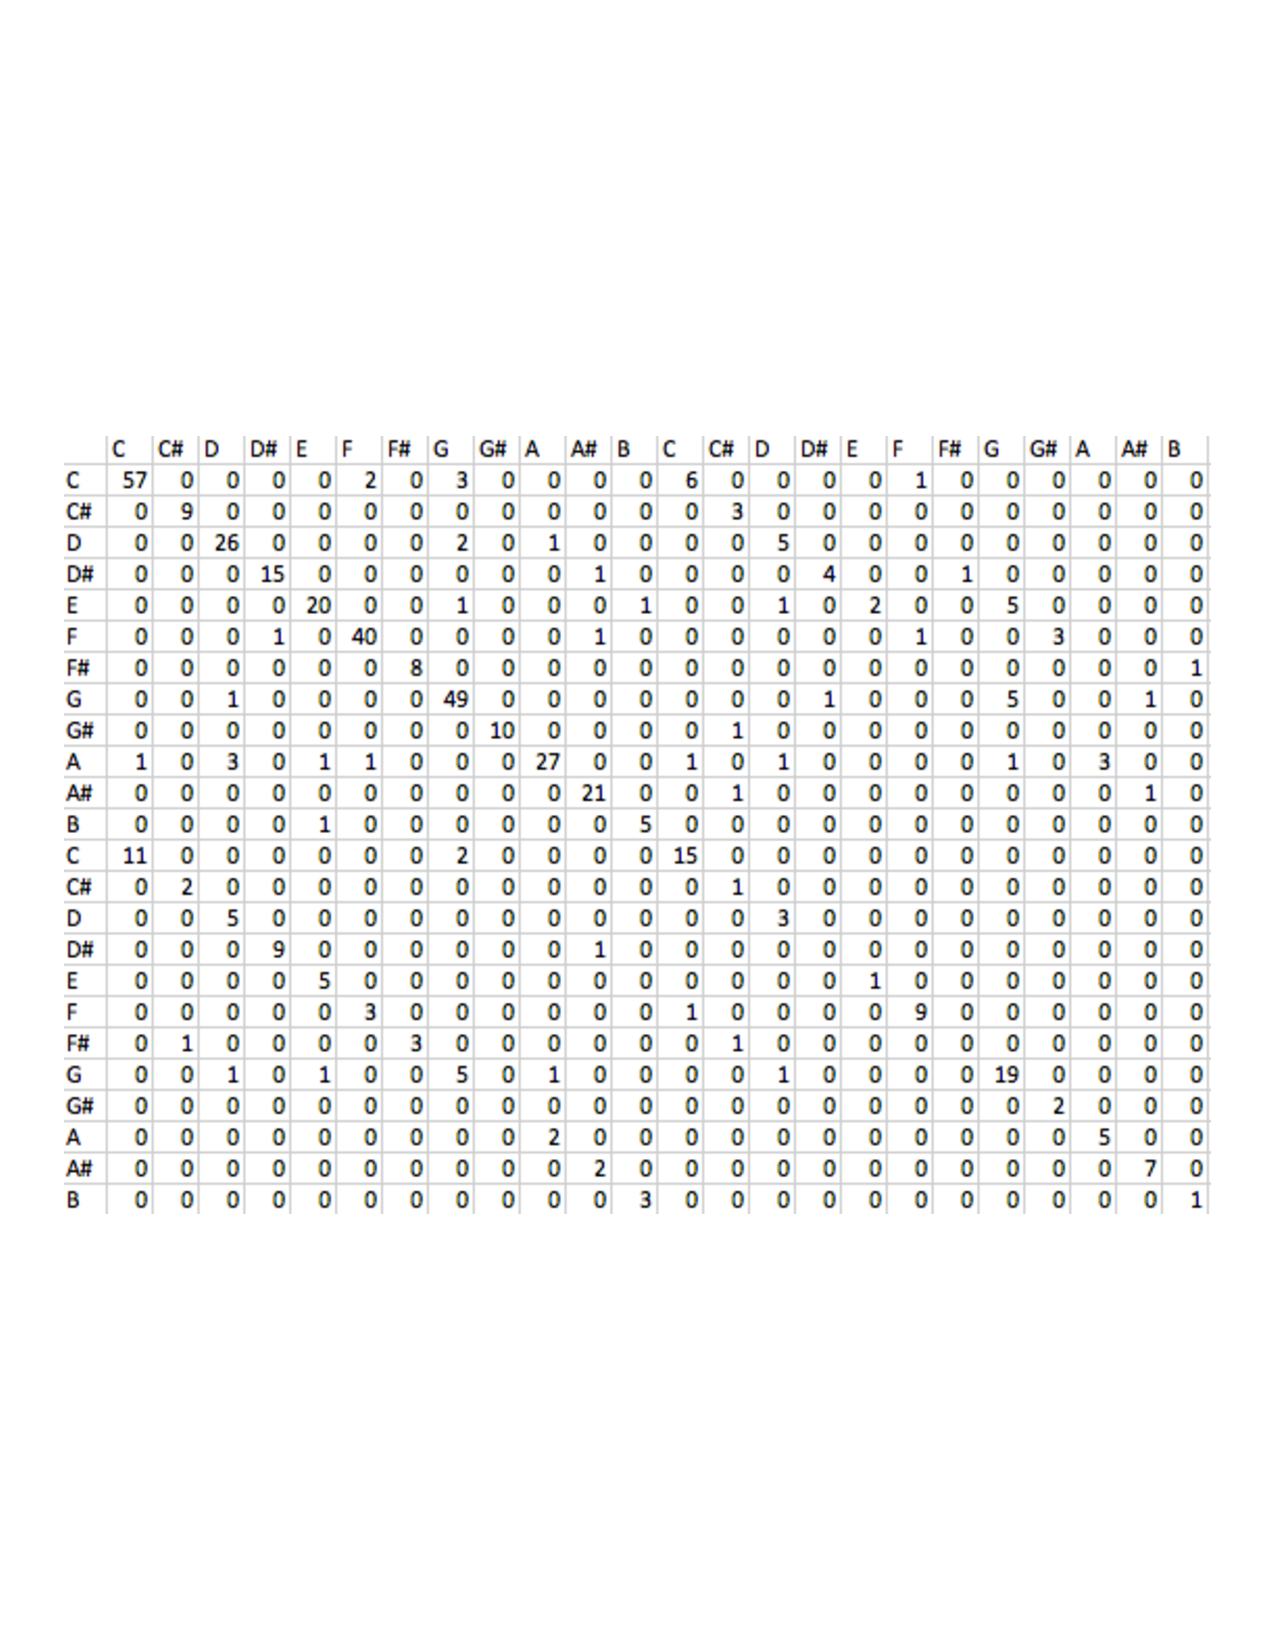
\includegraphics[width=\textwidth]{./confusion_matrix.pdf}
  \caption{\emph{Confusion Matrix for 4-gram model}. Much of the mis-classification confuses major and minor modes for the same key. In cases such as hard rock which use open fifths and exclude the third completely the mode (i.e., major or minor) is difficult to establish.}
  \label{fig:confusion_matrix}
\end{figure*}
``quote''
As regards the \emph{n}-gram models, we note that the unigram model is essentially equivalent to a pitch profile rendered as an applied probability distribution, and thus it seems reasonable that it should perform about on par with the RMSE of Pitch Count Profile method.

We increased the value of \emph{n} until we observed a decrease in accuracy. As is typical of \emph{n}-gram models, as \emph{n} increases, the model begins to essentially memorize more than can be generalized from the training data to the test data at which point the differences between instances become as significant as the differences between the key classes.

It is important to note that although our best accuracy on key-finding (.729) is significantly below the values reported by studies mentioned in the related works, the task of inferring key from melody is significantly more challenging than inferring key from songs which include harmony. It should also be considered that human listeners that are familiar with a melody may more accurately infer key from having familiarity with the harmony also. We therefore express confidence in the reported accuracies of these models.

Our results suggest that considering pitch counts or durations is less effective than a model which considers the sequence of pitches. This agrees with our intuition insofar as many pop songs spend the bulk of their duration modulating through chords which are not the root and may not even be closely related to the root. Notions of resolution and finding where the song ``lands'' inherently suggest that the contour and progression of the notes matters more than their frequency. The key is often most clearly defined at the beginning and ends of musical phrases or the beginning and end of the song itself. Whereas the method of counting note frequencies fails to give higher weight to these defining regions of the melodic passage, this information is embedded within the probabilistic framework of \emph{n}-gram models.

We find the superior accuracy of \emph{n}-gram models to the MuseScore key-signature inference model to be particularly promising inasmuch as it suggests that an \emph{n}-gram model might be used to improve the state of the art in industrial MIDI-reading software.

As regards key inference from monophonic pop melodies, we find that machine learning methods (\emph{n}-gram language models in particular) perform better than traditional key-finding algorithms, though both improve upon baseline accuracy. In the future we hope to evaluate how well unbiased human listeners would perform on the same task. We also envision developing a framework for detecting key \emph{changes} in pop melodies and for normalizing unlabeled melodic data for compositional analysis. 

\subsection{Verse-Chorus Inference}
\subsection{Rhyme Scheme}

\section{Discussion}

\section{Conclusion}

\bibliographystyle{iccc}
\bibliography{bib}

\end{document}